\documentclass{article}
\usepackage{listings}
\usepackage{hyperref}
\usepackage[T1]{fontenc}
\usepackage{txfonts}


\usepackage{graphicx}
\graphicspath{{./images/}}

\title{Quartus and QuestaSim - Tutorial \\ Reconfigurable Computing - Fall 2023 \\ University of Windsor}
\date{}
\author{Roche Christopher, Dr. Mohammed Khalid}


\begin{document}
	
	\maketitle
	\section{Introduction}
	This tutorial is intended to acquaint oneself with Quartus Prime Lite, Questasim and VHDL. A 4-bit adder will be implemented and simulated using VHDL in quartus and questasim. Pictorial represenation of the hardware model that we will be implementing is given below.
	
	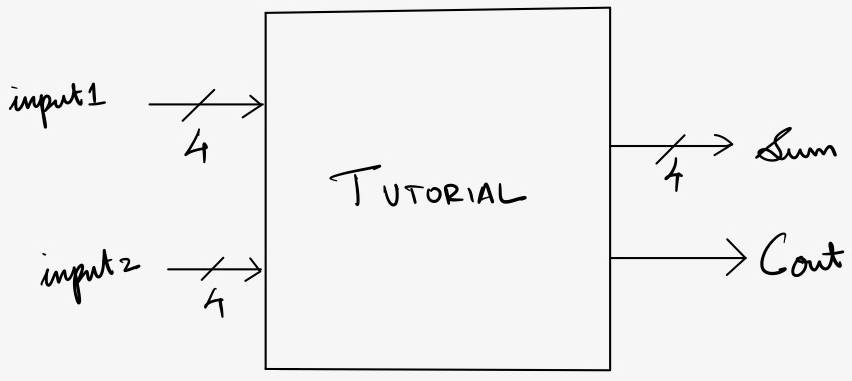
\includegraphics{rc_tutorial_entity_diagram.jpg}
	
	The model has 2 4-bits inputs, \textit{input1} and \textit{input2}, a 4-bits output \textit{sum} and a single bit output, \textit{cout}. The model performs binary addition on the two inputs and sets the output to \textit{sum} and if there is an overflow, the \textit{cout} port is set to high.
	
	\section{Quartus Prime Lite Software}
	\subsection{Setting up the project in Quartus Prime}
	\begin{enumerate}
		\item Open the quartus prime software 
		\item Create a new project.
		\begin{enumerate}
			\item Click \textbf{New Project Wizard} under \textbf \textbf{File}
			\item Click \textbf{Next} in the wizard, Enter the name of the project (eg. \textit{tutorial}) and click \textbf{Next}
			\item Select \textbf{Empty Project} and click \textbf{Next} twice
			\item Click the \textbf{Board} tab at the top, select \textbf{MAX 10} as Family, select \textbf{MAX 10 DE10-Lite} and click \textbf{Next}
			\item Select \textbf{Questa Intel FPGA} as Simulation Tool and \textbf{VHDL} as format.
			\item Click \textbf{Next} and click \textbf{Finish}.
		\end{enumerate}
	\end{enumerate}
	\subsection{Coding and Compilation}
	\begin{enumerate}
		\item Create a new VHDL file
		\begin{enumerate}
			\item Click \textbf{New} under \textbf{File}
			\item Select \textbf{VHDL file} under \textbf{Design Files} in the new wizard.
		\end{enumerate}
		\item Write the following code in the VHDL file and save it as \textit{tutorial.vhdl}
		
		\lstset{language=vhdl,
		tabsize=3,
		basicstyle={\small\ttfamily}}
		\begin{lstlisting}
		library ieee;
		use ieee.std_logic_1164.all;
		use ieee.numeric_std.all;
		use ieee.std_logic_unsigned.all;
		
		entity tutorial is
		port(
			input1, input2: in std_logic_vector(3 downto 0);
			sum: out std_logic_vector(3 downto 0);
			cout: out std_logic
		);
		end entity;
		
		architecture arch of tutorial is
			signal output_signal: std_logic_vector(4 downto 0);
			begin
				process(input1, input2)
				begin
					output_signal <= ('0' & input1) + ('0' & input2);
				end process;
				
				process(output_signal)
				begin
					sum <= output_signal(3 downto 0);
					cout <= output_signal(4);
				end process;
		end architecture;
		\end{lstlisting}
		\item Click \textbf{Start Compilation} under \textbf{Processing} tab.
	\end{enumerate}
	\section{Simulation using QuestaSim}
	\begin{enumerate}
		\item Compile the \textit{vhdl} file
		\begin{enumerate}
			\item Make sure the \textbf{Project} tab is selected, not the \textbf{Library} tab, in the left bottom section of the window.
			\item Right click the \textbf{vhdl} file, select \textbf{compile} option and click \textbf{compile selected}.
		\end{enumerate}
		\item Simulate using GUI
		\begin{enumerate}
			\item Click \textbf{Simulate} tab and click \textbf{Start Simulation}.
			\item A wizard will open and expand the \textbf{work} section. 
			\item Select the file to simulate, in our case it is \textit{tutorial}, and click \textbf{ok}
			\item The ports of the entity will be listed under the objects tab. Assign values to the input ports
			\begin{enumerate}
				\item Right click the object \textit{input1}, click \textbf{Modify}, select \textbf{Apply Wave}.
				\item In the wizard that opens up, set the \textit{Start Time} as \textbf{0}, \textit{Stop Time} as \textbf{100}, click \textbf{Next}, set the value to \textbf{0011} and click \textbf{Finish}. Now a wave window will appear with the \textit{input1} added to it.
				\item Right click the object \textit{input1} in the wave window, click \textbf{Edit}, select \textbf{Wave Editor} and click \textbf{Create/Modify Waveform}.
				\item In the wizard that opens up, set the \textit{Start Time} as \textbf{100}, \textit{Stop Time} as \textbf{200}, click \textbf{Next}, set the value to \textbf{1011} and click \textbf{Finish}
				
				\item Right click the object \textit{input2}, click \textbf{Modify}, select \textbf{Apply Wave}.
				\item In the wizard that opens up, set the \textit{Start Time} as \textbf{0}, \textit{Stop Time} as \textbf{200}, click \textbf{Next}, set the value to \textbf{1010} and click \textbf{Finish}.
			\end{enumerate}
			\item Add the waves of the output port to wave window.
			\begin{enumerate}
				\item Right click the \textit{output} object under the \textit{Objects} section and click \textbf{Add Wave}.
				\item Right click the \textit{overflow} object under the \textit{Objects} section and click \textbf{Add Wave}.
			\end{enumerate}
			\item Run the simulation
			\begin{enumerate}
				\item Click the \textit{Simulate} tab, Select \textit{Run} and click \textbf{Run -All}
			\end{enumerate}
		\end{enumerate}
		\item Simulate using testbench \\
		When the size of the project becomes bigger, simulating using graphical user interface becomes time consuming, cumbersome and virtually impossible. Testbench is preferred in scenarios such as those.
		\begin{enumerate}
			\item Create a file named \textit{tutorial\_tb.vhdl}
			\item Change the VHDL version to standard \textit{1076-2008}.
			\begin{enumerate}
				\item Right click \textit{tutorial\_tb.vhdl} and select \textbf{Properties}.
				\item Click \textbf{VHDL} tab, select \textbf{Use 1076-2008} and click \textbf{Ok}
			\end{enumerate}
			\item Copy the following testbench code to that file and compile it the way the vhdl model file was compiled.
			
			\lstset{language=vhdl,
					tabsize=3,
					basicstyle={\small\ttfamily}}
			\begin{lstlisting}
				library ieee;
				use ieee.std_logic_1164.all;
				use std.env.all;
				
				entity tutorial_testbench is
				end entity;
				
				architecture tut_testbench_arch of tutorial_testbench is
				
					component tutorial is
					port(
						input1, input2: in std_logic_vector(3 downto 0);
						sum: out std_logic_vector(3 downto 0);
						cout: out std_logic
					);
					end component;
					
					signal input1, input2, sum: std_logic_vector(3 downto 0);
					signal cout: std_logic;
					
					begin
						uut: tutorial
						port map(
						input1 => input1,
						input2 => input2,
						sum => sum,
						cout => cout
						);
						
						process
						begin
						input1 <= "1010";
						input2 <= "0011";
						wait for 5 ns;
						
						input1 <= "1000";
						input2 <= "1000";
						wait for 5 ns;
						
						input1 <= "1100";
						input2 <= "0011";
						wait for 5 ns;
						
						input1 <= "1111";
						input2 <= "0001";
						wait for 5 ns;
						
						stop(0);
					
					end process;
				end architecture;
			\end{lstlisting}
			\item Make sure that both the \textit{tutorial.vhdl} and \textit{tutorial\_tb.vhdl} exist in the same project. Then compile the programs by clicking \textbf{Compile} tab and \textbf{Compile All}.
			\item Click \textbf{Simulate} tab and click \textbf{Start Simulation}. Click \textbf{tutorial\_testbench} in the wizard and click \textbf{OK}.
			\item Under \textit{sim} tab, right click \textbf{tutorial\_testbench}, click \textbf{Add to}, click \textbf{Wave} and select \textbf{All items in region}. All waves should appear in the \textit{Wave} window.
			\item Click \textbf{Simulate} tab, select \textbf{Run} and click \textbf{Run -All}.
			
		\end{enumerate}
	\end{enumerate}

	\section{Appendix}
	The code attached in this document is available in the github repository, \url{https://github.com/rocheparadox/Reconfigurable-computing-fall-2023-quartus-tutorial}
\end{document}

